\documentclass{myslide}
\usepackage[slide]{mypackage}

\title{Computer System Architecture}
\subtitle{--- Digital Circuits}

\author[chhzh123]{陈鸿峥}
\date[Dec 30, 2018]{December, 2018}

\keywords{}

\begin{document}

\begin{frame}
\titlepage
\end{frame}

\begin{frame}
\tableofcontents[hideallsubsections]
\end{frame}

\section{基本概念}
\begin{frame}
\sectionpage
\end{frame}

\begin{frame}{计算机组成}
% 01.7-14
\begin{figure}
\centering
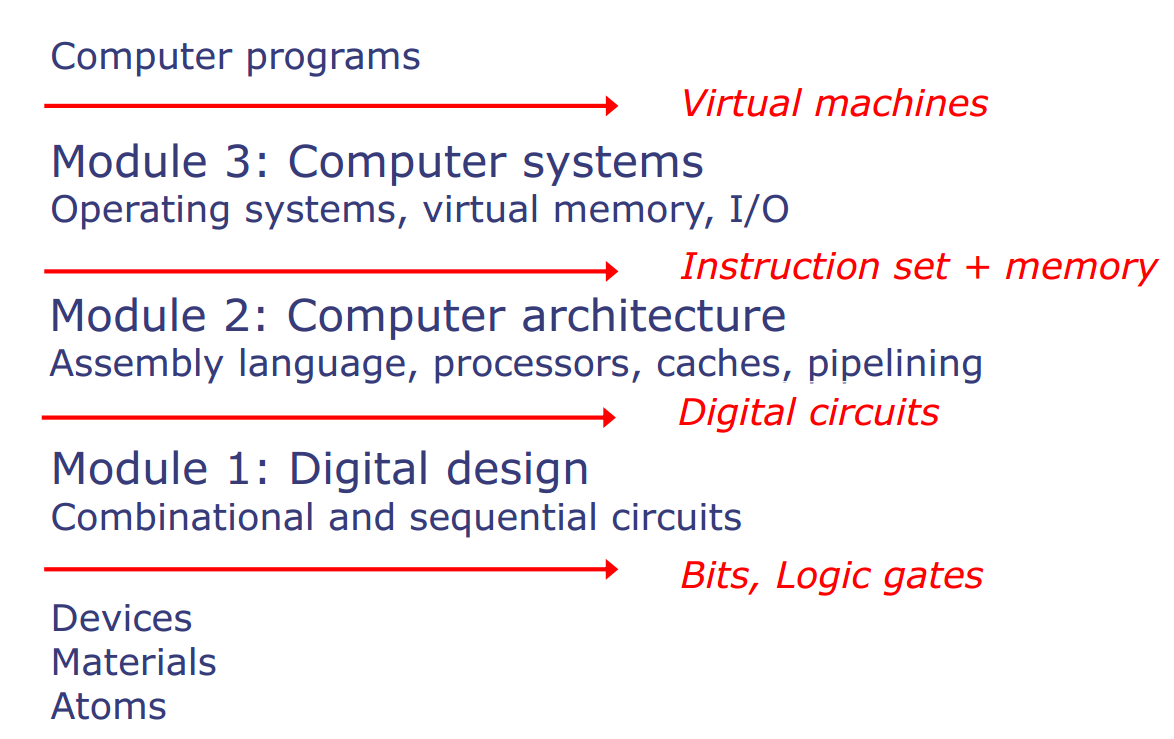
\includegraphics[width=\linewidth]{fig/organization.PNG}
\end{figure}
\end{frame}
% 01.22 Bluespec SystemVerilog流程

\begin{frame}{数字信号与模拟信号}
% 01.7-14
\begin{itemize}
	\item 模拟(analog)信号:连续
	\item 数字(digital)信号:离散,容许噪声,存在噪声容限(margin)
\end{itemize}
\begin{figure}
\centering
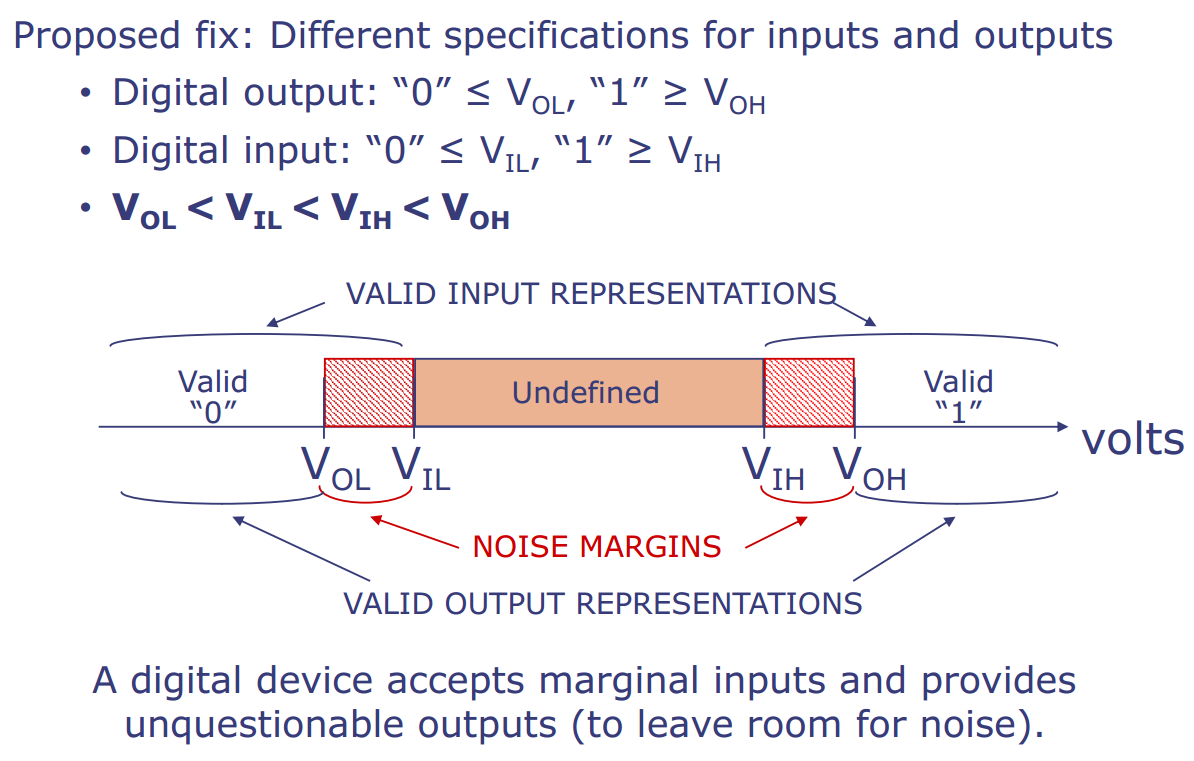
\includegraphics[width=0.8\linewidth]{fig/noise_margin.PNG}
\end{figure}
\end{frame}

\begin{frame}{数字模拟信号对比}
\begin{figure}
\centering
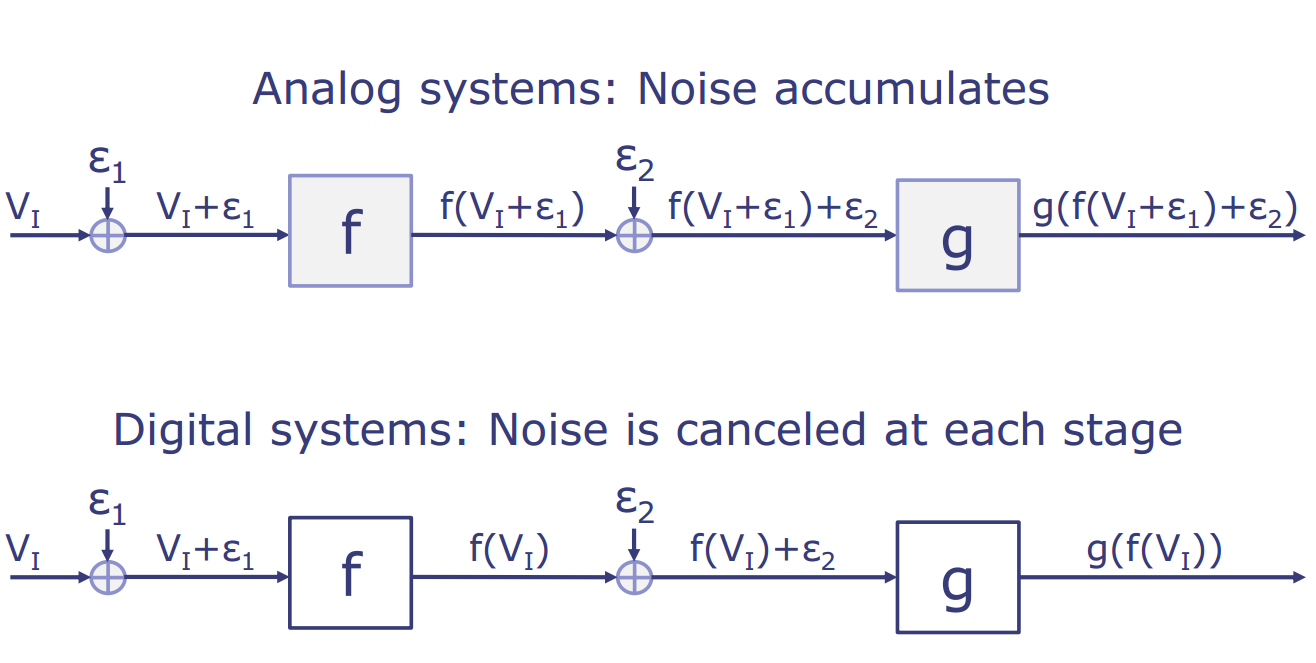
\includegraphics[width=\linewidth]{fig/digit_analog_comparison.PNG}
\end{figure}
\end{frame}

\begin{frame}{数字电路}
\begin{figure}
\centering
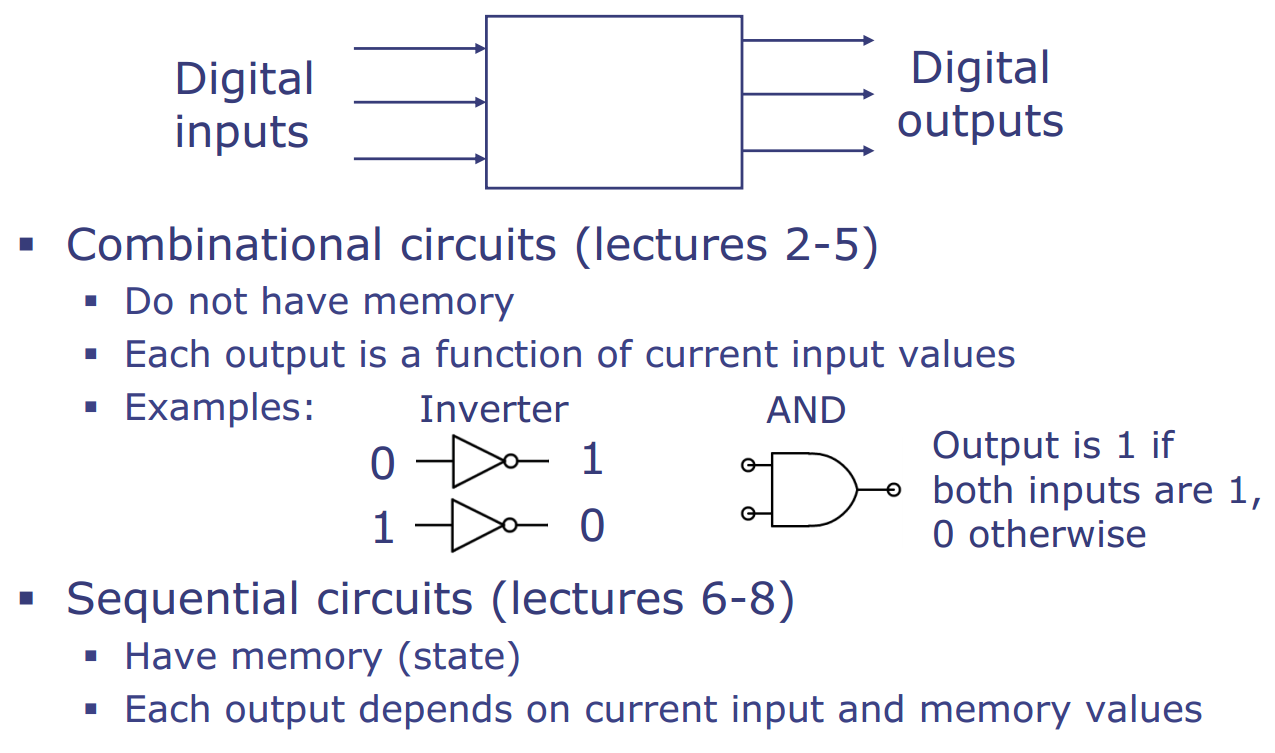
\includegraphics[width=\linewidth]{fig/type_of_digital_circuits.PNG}
\end{figure}
\end{frame}

\begin{frame}{布尔代数}
\begin{figure}
\centering
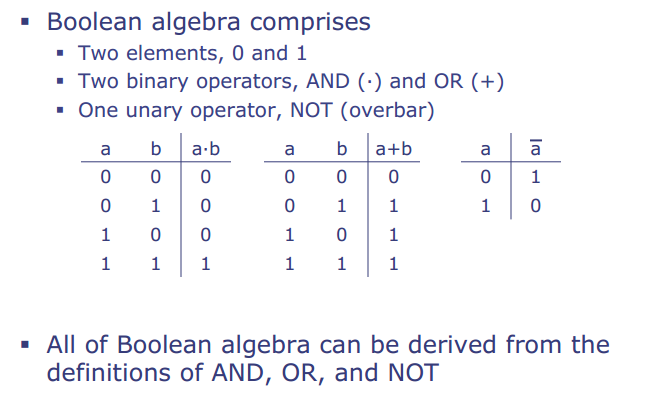
\includegraphics[width=\linewidth]{fig/boolean_algebra.PNG}
\end{figure}
\end{frame}

\begin{frame}{布尔代数公理}
\begin{figure}
\centering
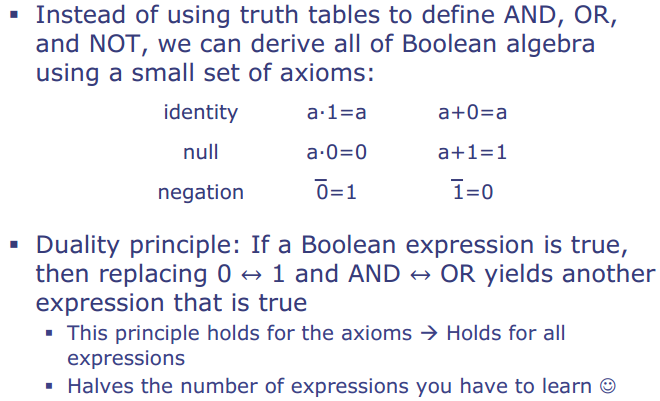
\includegraphics[width=\linewidth]{fig/boolean_algebra_axioms.PNG}
\end{figure}
\end{frame}

\begin{frame}{布尔代数性质}
\begin{figure}
\centering
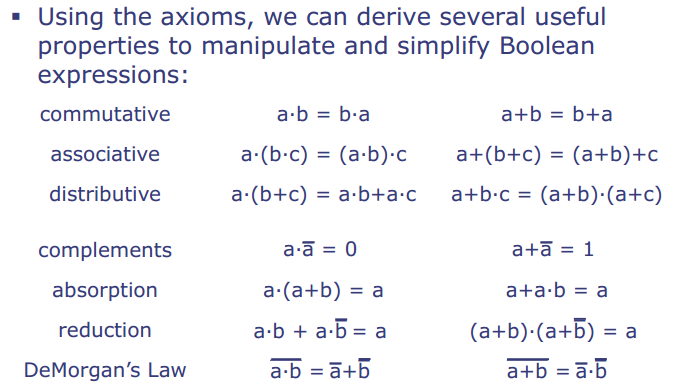
\includegraphics[width=\linewidth]{fig/boolean_algebra_law.PNG}
\end{figure}
\end{frame}

\begin{frame}{逻辑门}
\begin{figure}
\centering
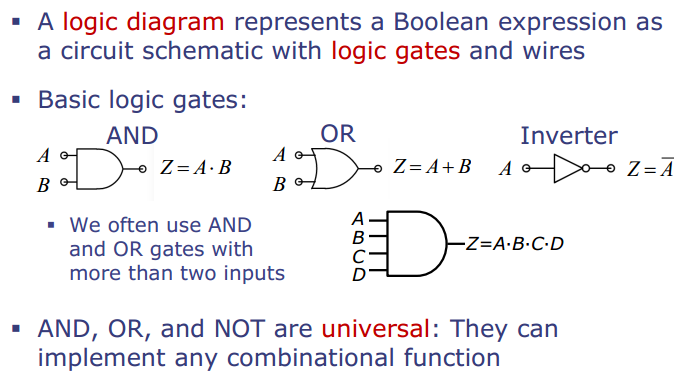
\includegraphics[width=\linewidth]{fig/boolean_to_logic_gate.PNG}
\end{figure}
\end{frame}

\begin{frame}{设计的折衷:时延与面积}
\begin{figure}
\centering
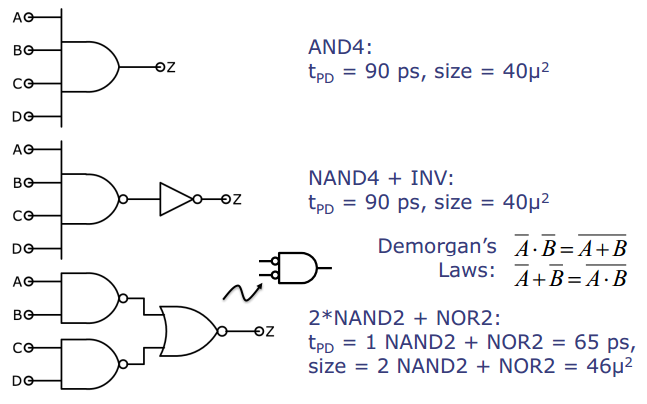
\includegraphics[width=\linewidth]{fig/delay_vs_size.PNG}
\end{figure}
\end{frame}

\end{document}